\chapter{Conceptual System Design}
The conceptual system design represents the structure of the system. It contains the conceptual model of the back end. The front end is only a module in this design to make the system design more simple. The front end design depends on which software architecture pattern is used. This project follows the MVC pattern \see{mvc}. In this chapter I introduce the system design and the general MVC pattern. The front end design will be introduced in \refstruc{frontend-system-design}, because it depends on the framework's behavior.

\section{System Design}

\todo{\% előkeresni a régi ábrát!!!! az újban 85\% Bence 15\%én - rendszertervezés email Bence okt 21}

The main components are the followings:

\begin{itemize}
	\item \textbf{Client:} A web portal, that is the communication bridge between the user and the web server. There will be three different modules: student, teacher and administrator. The different client modules can only communicate with the web server, and they cannot communicate with each other.
	\item \textbf{Database:} A database to store the system's data \see{ER-model}. 
	\item \textbf{Git:} A database to store the students' homeworks. Every student will get a different git repository for each laboratory.
	\item \textbf{Load Balancer:} It prevents the client from contacting the web server directly and solves the scalability problem. The client sends its requests to the load balancer, that will forward it to one of the web servers, depending on the client module, request type and the web servers' load.
	\item \textbf{Object-relational mapping:} It converts the data between the representation suitable for the implementation and the database. 
	\item \textbf{Messaging:} A component, that supports messaging between the different components. The web server, the task manager and the workers will use this to send tasks to each other.
	\item \textbf{Task Manager:} A special worker. It gets tasks from the web server to decide which worker has to process it. After the decision it forwards the task through the message bus.
	\item \textbf{Web Server:} The server that runs the API's implementation. This component processes the incoming requests, creates tasks and forwards them to the task manager. It also provides its clients the data from the databases. The API is written in Ruby on Rails. 
	\item \textbf{Worker:} This will process the task, e.g., changes the user's mailing list subscription.
\end{itemize}

\subsubsection{Scalability}

\newparagraph{Client}
To solve the scalability problem, the client's code will run in a web browser for every user. This way, resources for the client's code are provided by the user as he opens the web portal in a web browser.
 
\newparagraph{Web Server}
If there were not any load balancer between the client and the web server, then one server would get every request. With thousands of users this could lead to overload and high the response time. With a load balancer, the requests will first arrive at the load balancer, and it will decide which web server will handle that request and forwards it to that web server. The choice depends on the client module, request type and the web servers' load. The load balancer's purpose is to avoid overload and minimize the response time.
 
 \begin{figure}[!htbp]
 	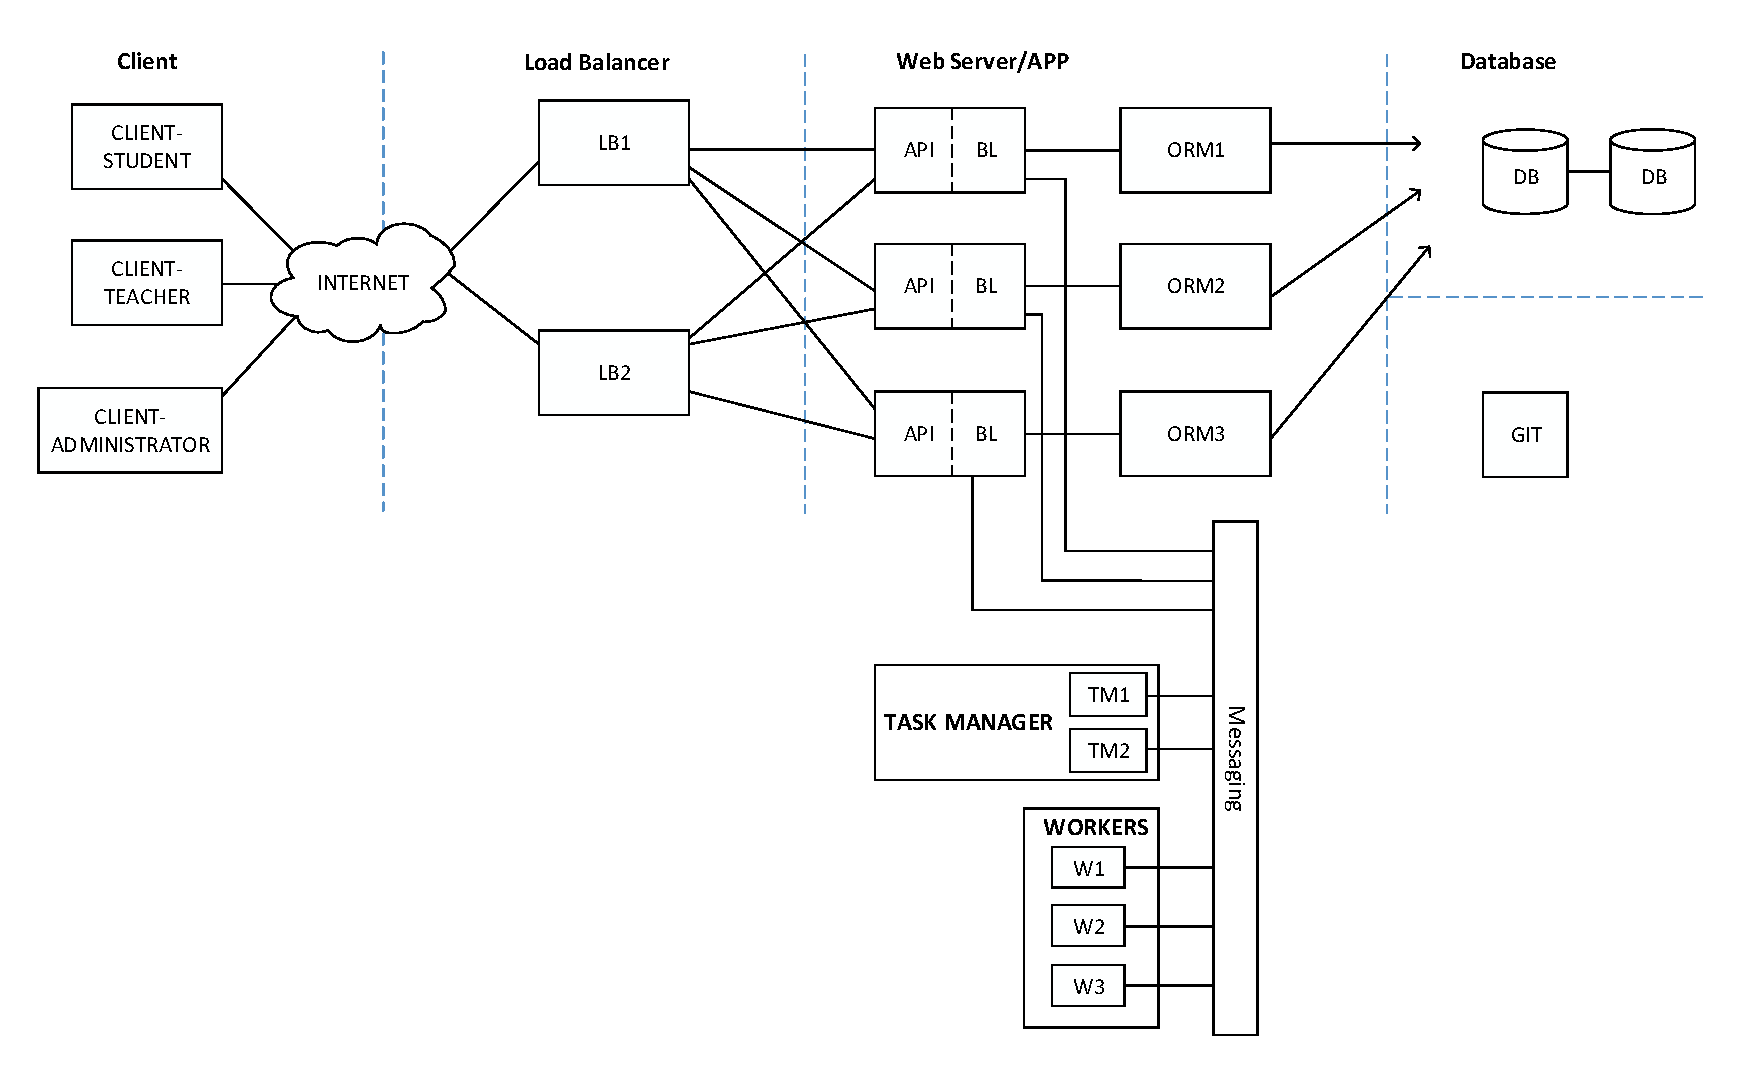
\includegraphics[width=0.95\textheight, angle=90]{figures/atfogo_rendszerterv_teljes.pdf}
 	\caption[Conceptional System Design]{Conceptional System Design}
 	\label{fig:conceptional-system-design}
 \end{figure}
 
 
 \todo{valamit nem kéne írni a biztonságról? adatok közötti átmenet, volt valami ilyesmi ábra asszem, meg hogy az LB eltakarja a rendszer felépítését a klienstől}
 
 \newpage
\subsection{Entity–Relationship Model}
\label{ER-model}

A data model describes the structures in which the database stores the data. The \emph{Entity-Relationship model} is a data model, that describes the data structure with entities and the relationships between them. An \emph{entity} is an existing information, that needs to be modeled. A \emph{property} is a qualifier, that makes the entities unique. A \emph{relationship} describes a connection between entities~\cite{adatb}.
 
The project's model uses Chen's notation. About 65 percent of the model was created by me, 35 percent of it was created by József Marton and it was finalized by the team. The attribute list is in \ref{attribute-list}.

 The main entities are the followings:

\begin{itemize}
	\item \textbf{Appointments:} An appointment connects the student groups with a date and a location.
	\item \textbf{Courses:} The courses, that use the portal.
	\item \textbf{Deliverables:} The way the students submit their homework. 
	\item \textbf{Deliverables/Repositories:} The repository, where students commit their source codes. 
	\item \textbf{Deliverables/Files:} The files, that students submit as homeworks. 
	\item \textbf{DeliverableTypes:} Describes the type of the submitted homework, e.g. documentation or git repository. 
	\item \textbf{Events:} An educational event is a class with a date for students	to participate.
	\item \textbf{EventTypes:} An event can be any type of class: lecture, laboratory or seminar. The Software Laboratory course has only laboratories.
	\item \textbf{ExerciseCategories:} Describes the type of the laboratory: DBMS, SQL, JDBC, X* or SOA.
	\item \textbf{ExerciseTypes:} Describe the topic and the language of the exercises. 
	\item \textbf{RegisteredStaffs:} A many-to-many relationship between the Semesters and the Staffs. It describes the staff member's role in the semester.
	\item \textbf{RegisteredStudents:} A many-to-many relationship between the Semesters and the Students. It describes which Neptun course is registered for a student in the semester.
	\item \textbf{Semesters:} The semester, when the course is being held.
	\item \textbf{StudentGroups:} In Software Laboratory 5 the students are separated into different groups. A group has one demonstrator and about 20 students.
	\item \textbf{Users:} The people, that use the portal during a semester.
	\item \textbf{Users/Staffs:} A type of user, who is not a student. This user can be an administrator and/or a demonstrator and/or an evaluator.
	\item \textbf{Users/Students:} A type of user, who attends the laboratories and solves a list of tasks.
\end{itemize}

\begin{figure}[!htbp]
	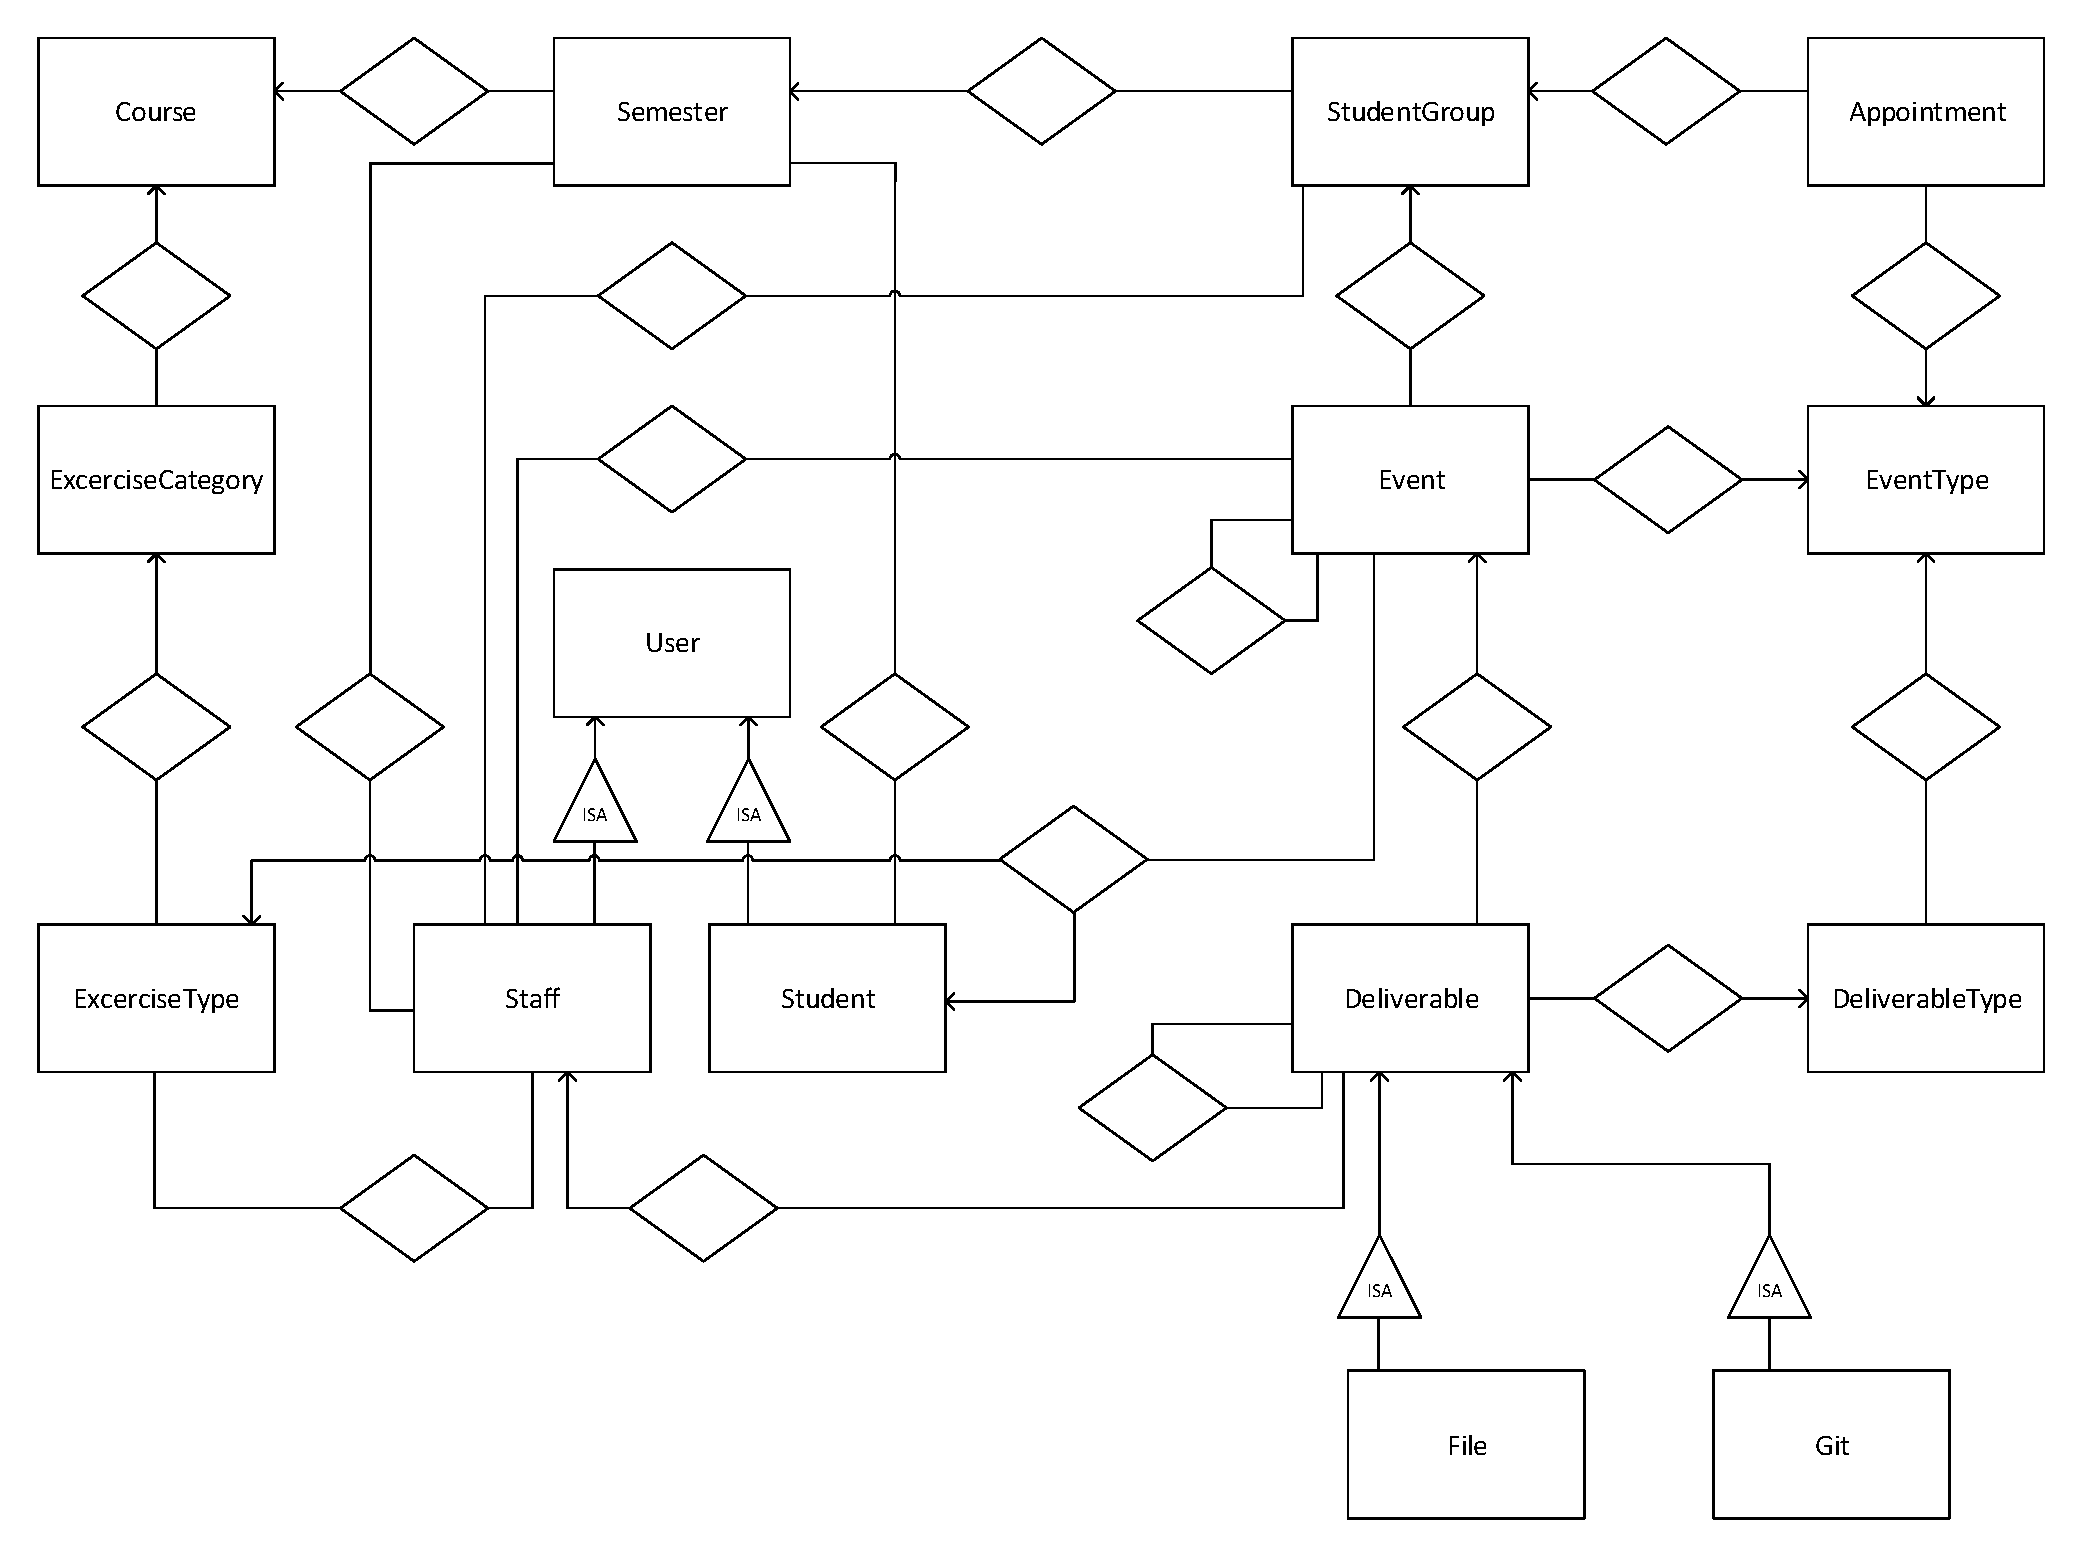
\includegraphics[width=0.85\textheight, angle=90]{figures/ER.pdf}
	\caption[Entity–relationship model]{Entity–relationship model}
	\label{fig:er}
\end{figure}

\newpage
\section{MVC Pattern}
\label{mvc}

The Model-View-Controller (MVC) is a software architecture pattern for user interface implementation, where the application logic is separated from the user interface.

In object-oriented programming the Model is the objects where the data from the database is stored. The View is the presentation layer. The user sees and interacts with the View. The Controller will process and respond to the user requests and invoke the changes in the Model. 

The MVC pattern is memory efficient, because multiple views can share the same underlying data model. Controllers can be separated by events. This allows the developer to create a controller hierarchy, because a controller for a keyboard event is different from a controller for a mouse event. Views implement an instance of a controller, that can be changed at run-time, because we can be disabled and enabled.

\subsection{MVC Web Applications}


\begin{figure}[!ht]
	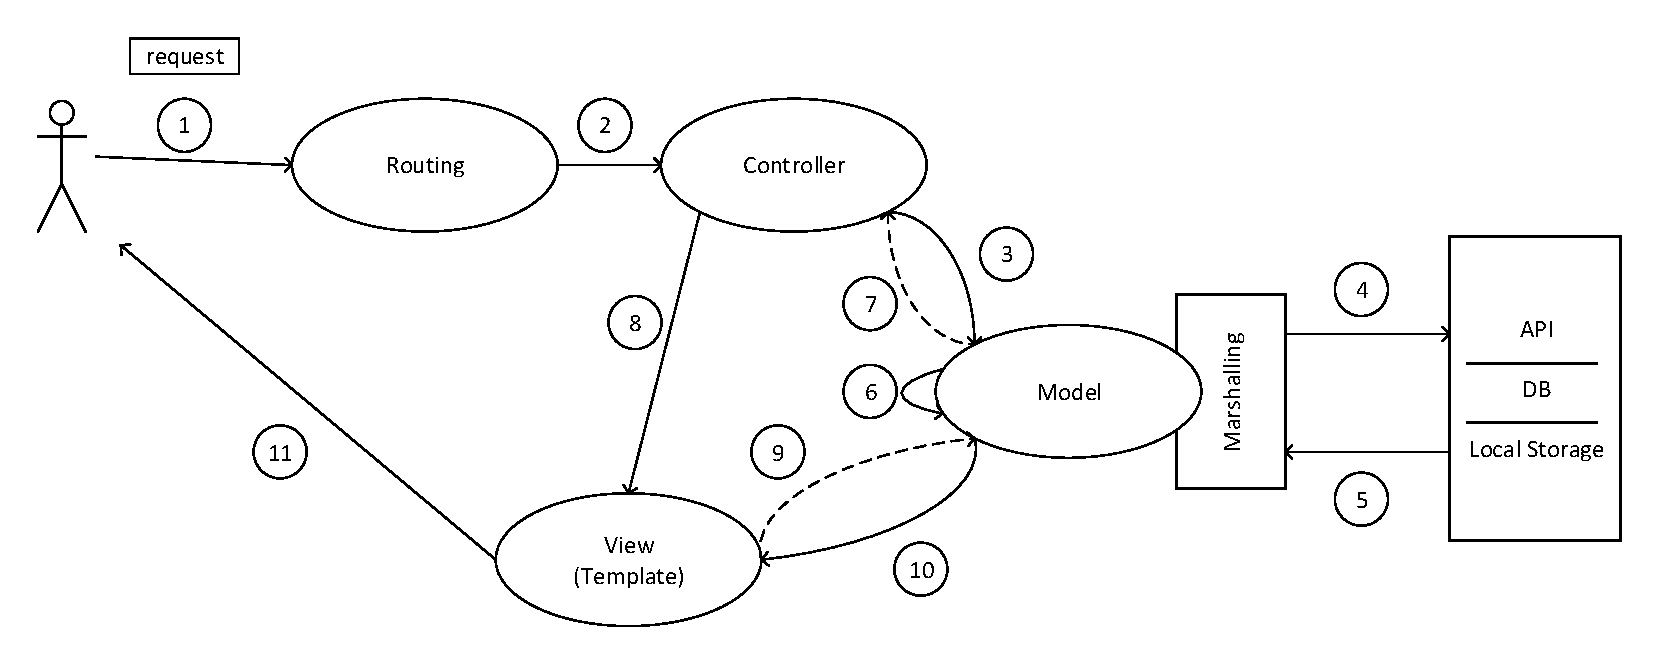
\includegraphics[width=\textwidth]{figures/klasszikus_mvc_webalkalmazas.pdf}
	\caption[Classic MVC Web Application]{Classic MVC Web Application\\Made by Bence Golda.}
	\label{fig:classic-mvc-webapplication}
\end{figure}

In web applications the browser communicates with a controller. When the user sends a request, routing will decide which controller will handle the request. The chosen controller talks to the model to get the relevant data. If it is necessary, the model will send data to or ask for data from the database, the API or the local storage. During this process, the data has to be transformed via marshalling. Marshalling is the process, that transforms the data between storable and sendable dataformats. When the model returns the desired data to the controller, it will forward the data to the view. The presentation layer will decide which page has to be returned to the browser, binds the data to the view template and returns it.


